\documentclass[11pt,letterpaper,twocolumn]{article}

\usepackage{graphicx}
\usepackage{hyperref}
\topmargin=-1in
\evensidemargin=0in
\oddsidemargin=0in
\textwidth=6.5in
\textheight=9.0in
\headsep=0.25in

\begin{document}

\title{Parcial No. 1}
\author{Sebastien Escobar}
\maketitle


\renewcommand{\abstractname}{Pregunta 1}
\begin{abstract}
Para solucionar este problema debemos de sustituir cada uno de los trozos de tierra por un punto y cada puente por un trazo.
\\
\\Esto crea un esquema simplificado el cual esta representado por las figuras adjuntas.
\\
\\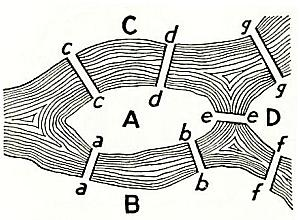
\includegraphics[height=3.5cm]{1}
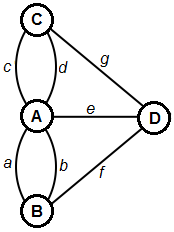
\includegraphics[height=3.5cm]{2}
\\
\\Como siguiente punto se hace una modelacion del grafo a partir de sus nodos y vertices.
Para ello se conforma el conjunto de nodos sobre el grafo:
\\
\\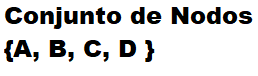
\includegraphics[height=1.5cm]{3}
\\La modelacion de los nodos nos sirve para implementar los puentes los cuales son los trazos semicirculares que se encuentran en la grafica de arriba. 
\\
\\Dichos trazos se comportan como los vertices de nuestro grafo. Y estan representados de la siguiente manera.
\\
\\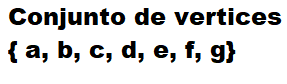
\includegraphics[height=1.5cm]{4}
\\Este tipo de vertices aunque a simple vista parezcan nodos estan compuestos por una pareja ordenada.
\\
\\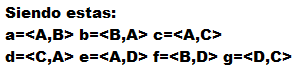
\includegraphics[height=2cm]{5}
\end{abstract}

\renewcommand{\abstractname}{Pregunta 2}
\begin{abstract}
Demostrar por induccion que la siguiente exprecion es correcta:
\\
\\$$\sum_{i=1}^{n} i = \frac{n(n+1)}{2}$$\\
\\Donde  $\sum_{i=1}^{n} i = 1+2+3+4+ \ldots +n$\\~\\
\\Demostrando que para nuestro caso base $i=1$ esta exprecion es correcta:
\\
\\$\sum_{i=1}^{n} i = \frac{n(n+1)}{2} = \frac{1(1+1)}{2} = 1$\\~\\
\\Entonces procedemos a utilizar nuestra suposicion:
\\$\sum_{i=1}^{n+1} i = \frac{n+1((n+1)+1)}{2}$\\~\\
\\Asumiendo que 
\\$\sum_{i=1}^{n} i = 1+2+3+4+ \ldots +n = \sum_{i=1}^{n} i = \frac{n(n+1)}{2}$\\~\\
\\
\\Pregunta 2
\\
\\Entonces $\sum_{i=1}^{n} i = 1+2+3+4+ \ldots +n+(n+1) = \sum_{i=1}^{n} i = \frac{n(n+1)}{2}+(n+1)$\\~\\
\\$= \frac{n(n+1)}{2}+\frac{2(n+1)}{2}$\\~\\
\\$= \frac{n(n+1)+2(n+1)}{2}$\\~\\
\\$= \frac{n+1((n+1)+1)}{2}$\\~\\
\end{abstract}

\renewcommand{\abstractname}{Pregunta 4}
\begin{abstract}
Para demostrar la conmutatividad de la suma. Empezaremos con el caso base: 
\\
\\Demostramos que, 
\begin{center}
P(0): a + b = b + a
\\P(0): 0 + b = b, b + 0 = b.
\end{center}

Ahora, por induccion suponemos que 
\begin{center}
P(a): a + b = b + a
\end{center}

Por el paso inductivo llegamos a, 
\begin{center}
P(s(a)): s(a) + b = b + s(a)
\end{center}

Tomando el lado derecho:
\begin{center}
b + s(a)= s(b + a)= s(a + b)
\end{center}

Ya que conocemos la definicion de la suma de numeros naturales podemos pasarnos su demostracion y llegar a:
\\
\begin{center}
\textbf{s(a + b)= s(a) + b}
\end{center}
\end{abstract}
\renewcommand{\abstractname}{Pregunta 5}
\begin{abstract}
Dada la funci\'on $a\geq b$ para numeros naturales unarios:
\[
        a\geq b =
                \left\{
                        \begin{array}{ll}
                                s(o)  & \mbox{si } b = o \\
                                o & \mbox{si } a = o \\
                                i\geq j & \mbox{si } a = s(i)\ \&\ b = s(j)
                        \end{array}
                \right.
\]
Para este caso, 
\\empezamos con un caso base: n=0
\begin{center}
Donde ((0+0) $ \geq $ 0)
\\
 0 + 0 = 0, 0 $\geq$ 0
\end{center}
Asumimos para el caso inductivo que n = s(0)
\\ Si hacemos unas sustituciones llegamos a:
\begin{center}
((s(0)+s(0)) $\geq$ s(0))
\end{center}
Asumiendo la conmutatividad de la suma, podemos expresarlo como:
\begin{center}
((s(s(0+0))) $\geq $ s(0))
\\((s(s(0))) $\geq $ s(0))
\\(s(s(0)) - s(0) $\geq$ 0)
\\(s(0) $\geq$ 0)
\end{center}
Llegando asi a: 
(((n+n) $\geq$ n) = s(0)) = s(0)
\end{abstract}

\end{document}